\documentclass[mstat,12pt]{unswthesis}

\usepackage{color}
\usepackage{fancyvrb}
\newcommand{\VerbBar}{|}
\newcommand{\VERB}{\Verb[commandchars=\\\{\}]}
\DefineVerbatimEnvironment{Highlighting}{Verbatim}{commandchars=\\\{\}}
% Add ',fontsize=\small' for more characters per line
\usepackage{framed}
\definecolor{shadecolor}{RGB}{248,248,248}
\newenvironment{Shaded}{\begin{snugshade}}{\end{snugshade}}
\newcommand{\AlertTok}[1]{\textcolor[rgb]{0.94,0.16,0.16}{#1}}
\newcommand{\AnnotationTok}[1]{\textcolor[rgb]{0.56,0.35,0.01}{\textbf{\textit{#1}}}}
\newcommand{\AttributeTok}[1]{\textcolor[rgb]{0.13,0.29,0.53}{#1}}
\newcommand{\BaseNTok}[1]{\textcolor[rgb]{0.00,0.00,0.81}{#1}}
\newcommand{\BuiltInTok}[1]{#1}
\newcommand{\CharTok}[1]{\textcolor[rgb]{0.31,0.60,0.02}{#1}}
\newcommand{\CommentTok}[1]{\textcolor[rgb]{0.56,0.35,0.01}{\textit{#1}}}
\newcommand{\CommentVarTok}[1]{\textcolor[rgb]{0.56,0.35,0.01}{\textbf{\textit{#1}}}}
\newcommand{\ConstantTok}[1]{\textcolor[rgb]{0.56,0.35,0.01}{#1}}
\newcommand{\ControlFlowTok}[1]{\textcolor[rgb]{0.13,0.29,0.53}{\textbf{#1}}}
\newcommand{\DataTypeTok}[1]{\textcolor[rgb]{0.13,0.29,0.53}{#1}}
\newcommand{\DecValTok}[1]{\textcolor[rgb]{0.00,0.00,0.81}{#1}}
\newcommand{\DocumentationTok}[1]{\textcolor[rgb]{0.56,0.35,0.01}{\textbf{\textit{#1}}}}
\newcommand{\ErrorTok}[1]{\textcolor[rgb]{0.64,0.00,0.00}{\textbf{#1}}}
\newcommand{\ExtensionTok}[1]{#1}
\newcommand{\FloatTok}[1]{\textcolor[rgb]{0.00,0.00,0.81}{#1}}
\newcommand{\FunctionTok}[1]{\textcolor[rgb]{0.13,0.29,0.53}{\textbf{#1}}}
\newcommand{\ImportTok}[1]{#1}
\newcommand{\InformationTok}[1]{\textcolor[rgb]{0.56,0.35,0.01}{\textbf{\textit{#1}}}}
\newcommand{\KeywordTok}[1]{\textcolor[rgb]{0.13,0.29,0.53}{\textbf{#1}}}
\newcommand{\NormalTok}[1]{#1}
\newcommand{\OperatorTok}[1]{\textcolor[rgb]{0.81,0.36,0.00}{\textbf{#1}}}
\newcommand{\OtherTok}[1]{\textcolor[rgb]{0.56,0.35,0.01}{#1}}
\newcommand{\PreprocessorTok}[1]{\textcolor[rgb]{0.56,0.35,0.01}{\textit{#1}}}
\newcommand{\RegionMarkerTok}[1]{#1}
\newcommand{\SpecialCharTok}[1]{\textcolor[rgb]{0.81,0.36,0.00}{\textbf{#1}}}
\newcommand{\SpecialStringTok}[1]{\textcolor[rgb]{0.31,0.60,0.02}{#1}}
\newcommand{\StringTok}[1]{\textcolor[rgb]{0.31,0.60,0.02}{#1}}
\newcommand{\VariableTok}[1]{\textcolor[rgb]{0.00,0.00,0.00}{#1}}
\newcommand{\VerbatimStringTok}[1]{\textcolor[rgb]{0.31,0.60,0.02}{#1}}
\newcommand{\WarningTok}[1]{\textcolor[rgb]{0.56,0.35,0.01}{\textbf{\textit{#1}}}}


%%%%%%%%%%%%%%%%%%%%%%%%%%%%%%%%%%%%%%%%%%%%%%%%%%%%%%%%%%%%%%%%%%
% 
% OK...Now we get to some actual input.  The first part sets up
% the title etc that will appear on the front page
%
%%%%%%%%%%%%%%%%%%%%%%%%%%%%%%%%%%%%%%%%%%%%%%%%%%%%%%%%%%%%%%%%%

\title{Projet réalisé par\\[0.5cm] l'équipe GBSC du groupe de TD2 \\[3cm]Rapport
de groupe des UE \newline  Bases de données + Sciences des Données 2}

\authornameonly{Kardiatou BA, Lea CARMINATI, Diella Joannie GATEKA, Lana
SCHEMBRI. }

\author{\Authornameonly}

\copyrightfalse
\figurespagefalse
\tablespagefalse

%%%%%%%%%%%%%%%%%%%%%%%%%%%%%%%%%%%%%%%%%%%%%%%%%%%%%%%%%%%%%%%%%
%
%  And now the document begins
%  The \beforepreface and \afterpreface commands puts the
%  contents page etc in
%
%%%%%%%%%%%%%%%%%%%%%%%%%%%%%%%%%%%%%%%%%%%%%%%%%%%%%%%%%%%%%%%%%%


\input{header.tex}

\renewcommand{\contentsname}{Table des matières}

\renewcommand{\chaptername}{Chapitre}




\begin{document}

\beforepreface

%\afterpage{\blankpage}

% plagiarism

\prefacesection{Déclaration de non plagiat}

\vskip 2pc \noindent Nous déclarons que ce rapport est le fruit de notre seul travail, à part lorsque cela est indiqué  explicitement. 

\vskip 2pc  \noindent Nous acceptons que la personne évaluant ce rapport puisse, pour les besoins de cette évaluation:
\begin{itemize}
\item la reproduire et en fournir une copie à un autre membre de l'université; et/ou,
\item en communiquer une copie à un service en ligne de détection de plagiat (qui pourra en retenir une copie pour les besoins d'évaluation future).
\end{itemize}

\vskip 2pc \noindent Nous certifions que nous avons lu et compris les règles ci-dessus.\vspace{24pt}

\vskip 2pc \noindent En signant cette déclaration, nous acceptons ce qui précède.
\vskip 2pc \noindent

Signature: Kardiatou BA \hfill Date: 30/04/2025\\[0.5cm]
Signature: Lea CARMINATI \hfill Date: 30/04/2025 \\[0.5cm]
Signature: Diella Joannie GATEKA \hfill Date: 30/04/2025 \\[0.5cm]
Signature: Lana SCHEMBRI \hfill Date: 30/04/2025 \\[0.5cm]

\vskip 1pc

%\textcolor{red}{Mettre à jour la date.}

{\bigskip\bigskip\bigskip\noindent} \today
%\afterpage{\blankpage}

% Acknowledgements are optional


\prefacesection{Remerciements}

{\bigskip}Nous adressons nos plus sincères remerciements à nos
encadrantes pédagogiques, Mme Bringay et Mme Demangeot, pour leurs
précieux conseils, leur soutien constant et leur disponibilité tout au
long de la réalisation de notre projet. Leur expertise a été essentielle
pour le bon déroulement et le développement de notre travail.
\newline Nous leur sommes profondément reconnaissantes pour le temps et
l'énergie qu'elles ont consacrés à notre accompagnement, ainsi que pour
la passion avec laquelle elles nous ont transmis leurs
connaissances\\[1cm] 

{\bigskip\bigskip\bigskip\noindent} \today

%\afterpage{\blankpage}

% Abstract

\prefacesection{Résumé}

Nous sommes perpétuellement à la recherche du confort, de la
tranquillité, d'une meilleure qualité de vie en général. Cela peut
passer par le choix du département dans lequel on souhaite vivre, dans
l'espoir de s'y épanouir pleinement. On a souvent tendance à penser que
des revenus élevés, à l'échelle territoriale, sont synonymes de confort.
Mais est-ce réellement le cas ? \newline Notre rapport s'intéresse
particulièrement aux départements français. Pour évaluer la qualité de
vie qu'ils offrent, il nous a semblé pertinent d'analyser une série
d'indicateurs : des indicateurs socio-économiques, tels que le taux de
chômage et le taux de pauvreté ; socio démographiques et structurels,
comme la densité de population, le nombre d'habitants, le nombre total
de logements et le taux de logements sociaux ; et enfin, des indicateurs
culturels, comme le nombre d'établissements culturels par département.
\newline Le choix du département où l'on souhaite vivre parviendra-t-il
à satisfaire toutes nos attentes ? Après une étude approfondie de nos
données, nous avons pu constater que des revenus moyens élevés ne
garantissent pas forcément de meilleures conditions de vie. Certains
départements affichant des revenus salariaux élevés présentent également
des taux de chômage et de pauvreté non négligeables, une forte densité
de population et un grand nombre d'établissements culturels, mais aussi
des risques accrus de saturation des services publics. On y observe
souvent des inégalités sociales marquées, avec la coexistence de zones
très favorisées et d'autres en grande précarité, sans oublier un taux de
logements sociaux souvent insuffisant face à la demande. \newline À
l'inverse, certains départements économiquement moins favorisés offrent
parfois un cadre de vie plus équilibré : faible densité, pauvreté
modérée et bonne accessibilité aux infrastructures culturelles.
\newline D'ailleurs, pour appuyer nos propos, des tests statistiques de
corrélation ont permis de rejeter l'hypothèse d'une relation
significative entre le niveau de revenu salarial et les taux de chômage
ou de pauvreté. \newline Étant donné que le test d'ANOVA montre que le
revenu moyen d'un département à un effet significatif sur le nombre
d'établissements culturels. \newline Ainsi, ce rapport met en lumière la
complexité des dynamiques territoriales et la nécessité de dépasser les
simples critères économiques pour penser la qualité de vie.

%\afterpage{\blankpage}


\afterpreface





%%%%%%%%%%%%%%%%%%%%%%%%%%%%%%%%%%%%%%%%%%%%%%%%%%%%%%%%%%%%%%%%%%
%
% Now we can start on the first chapter
% Within chapters we have sections, subsections and so forth
%
%%%%%%%%%%%%%%%%%%%%%%%%%%%%%%%%%%%%%%%%%%%%%%%%%%%%%%%%%%%%%%%%%%



%%%%%%%%%%%%%%%%%%%%%%%%%%%%%%%%%%%%%

%\afterpage{\blankpage}


\chapter{Introduction}\label{introduction}

La qualité de vie est influencée par de nombreux facteurs, comme par
exemple les facteurs économiques, la répartition démographique et les
services publics. Quand on évalue le bien-être d'une population, on
pourrait penser qu'un revenu moyen élevé garantit de meilleures
conditions de vie. Cependant cette corrélation n'est pas évidente :
certains départements riches peuvent être confrontés à des
problématiques telles que des coûts de logements élevés, ou une forte
densité de population, tandis que d'autres, avec des revenus plus bas,
peuvent s'offrir un cadre de vie plus équilibré. Dès lors, nous pouvons
nous poser les questions suivantes : \bigskip

\begin{center}

\textbf{Les départements français offrants les meilleures conditions de vie sont-ils nécessairement ceux avec les revenus moyens les plus élevés?  Et ces départements se démarquent-ils du lot avec des infrastructures culturelles plus nombreuses et avec moins de logements sociaux?
}

\end{center}
\medskip

\justifying

Ces questions nous aident à comprendre les dynamiques entre revenu,
salaire, logement sociaux, nombre d'établissements culturels (cinéma,
théâtre, musée, etc) et bien-être social. En répondant à cette
problématique, nous pourrons identifier les critères qui définissent une
bonne qualité de vie. Comprendre ces dynamiques peut être utile aux
citoyens pour faire des choix de résidences plus conscientes, aux
politiques d'investissement et aménagement pour mieux s'orienter. Cette
analyse pourrait ainsi favoriser un développement territorial plus
équilibré et sensibiliser aux déterminants de la qualité de vie. En
croisant les données économiques et sociales, cette étude propose une
lecture plus nuancée des disparités sociales en France.

\section{Responsabilités et composition de
l'équipe}\label{responsabilituxe9s-et-composition-de-luxe9quipe}

\medskip

Kardiatou BA: Étudiant n° 22310777, Responsable de la collecte,
manipulation des données, rapport et de la partie base de données.

\medskip

Lea CARMINATI Étudiant n° 22307644, Responsable gestion rapport, de la
partie statistique.

\medskip

Diella Joannie GATEKA : Étudiant n° 22311183, Responsable de la
collecte, manipulation des données, rapport et de la partie base de
données.

\medskip

Lana SCHEMBRI: Étudiant n° 22313116, Responsable rapport de la partie
statistique.

\chapter{Base de données}\label{base-de-donnuxe9es}

\section{Provenance des données}\label{provenance-des-donnuxe9es}

Voici les sources de données utilisées pour notre travail:

\textbf{Source de données 1}:

\tiny

\texttt{\url{https://www.data.gouv.fr/fr/datasets/limpot-sur-le-revenu-par-collectivite-territoriale-ircom/}}
\normalsize (format xlsx,12 colonnes et 1897 lignes).

Ce premier jeu de données fournit des informations sur les revenus des
personnes vivant en France, réparties par département, sur la période de
2000 à 2017.

\bigskip

\textbf{Source de données 2}:

\tiny

\texttt{\url{https://www.data.gouv.fr/fr/datasets/logements-et-logements-sociaux-dans-les-departements-1/}}
\normalsize (format csv, 34 colonnes et 601 lignes).

Ce deuxième jeu de données permet d'analyser l'évolution des
territoires, l'activité de la construction et le secteur du logement
social. Il comprend également plusieurs indicateurs utiles pour évaluer
la qualité de vie dans les départements.

\bigskip

\textbf{Source de données 3}:

\tiny

\texttt{\url{https://www.data.gouv.fr/fr/datasets/entreprises-nombre-detablissements-culturels-actifs-par-departement/}}
\normalsize (format csv, 101 lignes et 5 colonnes).

Ce troisième jeu de données renseigne sur le nombre total
d'établissements culturels présents dans chaque département depuis 2022.
Il indique également, d'une part, le nombre d'établissements culturels
construits en 2018, et d'autre part, la part que ces établissements
représentent.

\medskip

La population étudiée correspond aux ménages français, répartis par
département, avec une distinction entre salariés et retraités. Les
données permettent d'analyser les disparités économiques et sociales
entre les territoires. Les revenus fournissent une vision des écarts
financiers, tandis que le chômage, la pauvreté et les logements
permettent d'évaluer la qualité de vie socio-économique. Les unités
statistiques sont les départements français. Ils offrent une échelle
d'analyse pour comparer les dynamiques sociales et économiques du pays.

\section{Descriptif des tables}\label{descriptif-des-tables}

Voici les tables conservées après filtrage:

\begin{longtable}[]{@{}
  >{\centering\arraybackslash}p{(\columnwidth - 6\tabcolsep) * \real{0.2326}}
  >{\centering\arraybackslash}p{(\columnwidth - 6\tabcolsep) * \real{0.1047}}
  >{\centering\arraybackslash}p{(\columnwidth - 6\tabcolsep) * \real{0.4651}}
  >{\centering\arraybackslash}p{(\columnwidth - 6\tabcolsep) * \real{0.1977}}@{}}
\caption{Departement (101 \(\times\) 13)}\tabularnewline
\toprule\noalign{}
\begin{minipage}[b]{\linewidth}\centering
Nom colonne
\end{minipage} & \begin{minipage}[b]{\linewidth}\centering
Type
\end{minipage} & \begin{minipage}[b]{\linewidth}\centering
Signification
\end{minipage} & \begin{minipage}[b]{\linewidth}\centering
Caractéristique
\end{minipage} \\
\midrule\noalign{}
\endfirsthead
\toprule\noalign{}
\begin{minipage}[b]{\linewidth}\centering
Nom colonne
\end{minipage} & \begin{minipage}[b]{\linewidth}\centering
Type
\end{minipage} & \begin{minipage}[b]{\linewidth}\centering
Signification
\end{minipage} & \begin{minipage}[b]{\linewidth}\centering
Caractéristique
\end{minipage} \\
\midrule\noalign{}
\endhead
\bottomrule\noalign{}
\endlastfoot
code\_dep & integer & code departement & clé primaire \\
nom\_dep & varchar & nom departement & \\
code\_region & integer & code region & clé étrangère \\
nbr\_hab & integer & nombre habitants departement & \\
densite & double & densite habitants departement & \\
pourcpopvingt & double & pourcentage population 20 ans & \\
pourpopsoixante & double & pourcentage population 60 ans & \\
taux\_chomage & double & taux de chômage departement & \\
taux\_pauvrete & double & taux pauvrete departement & \\
nbr\_foyer\_salarie & integer & nombre des foyers salariés departement
& \\
montant\_salairie & double & montant des salaires & \\
nbr\_foyer\_retraite & integer & nombre des foyers retraités & \\
montant\_retraite & double & montant des retraites & \\
\end{longtable}

\begin{longtable}[]{@{}cccc@{}}
\caption{Region (18 \(\times\) 2)}\tabularnewline
\toprule\noalign{}
Nom colonne & Type & Signification & Caractéristique \\
\midrule\noalign{}
\endfirsthead
\toprule\noalign{}
Nom colonne & Type & Signification & Caractéristique \\
\midrule\noalign{}
\endhead
\bottomrule\noalign{}
\endlastfoot
code\_region & integer & code region & clé primaire \\
nom\_region & varchar & nom region & unique \\
\end{longtable}

\begin{longtable}[]{@{}
  >{\centering\arraybackslash}p{(\columnwidth - 6\tabcolsep) * \real{0.1728}}
  >{\centering\arraybackslash}p{(\columnwidth - 6\tabcolsep) * \real{0.1111}}
  >{\centering\arraybackslash}p{(\columnwidth - 6\tabcolsep) * \real{0.5062}}
  >{\centering\arraybackslash}p{(\columnwidth - 6\tabcolsep) * \real{0.2099}}@{}}
\caption{Etablissement (101 \(\times\) 4) \medskip}\tabularnewline
\toprule\noalign{}
\begin{minipage}[b]{\linewidth}\centering
Nom colonne
\end{minipage} & \begin{minipage}[b]{\linewidth}\centering
Type
\end{minipage} & \begin{minipage}[b]{\linewidth}\centering
Signification
\end{minipage} & \begin{minipage}[b]{\linewidth}\centering
Caractéristique
\end{minipage} \\
\midrule\noalign{}
\endfirsthead
\toprule\noalign{}
\begin{minipage}[b]{\linewidth}\centering
Nom colonne
\end{minipage} & \begin{minipage}[b]{\linewidth}\centering
Type
\end{minipage} & \begin{minipage}[b]{\linewidth}\centering
Signification
\end{minipage} & \begin{minipage}[b]{\linewidth}\centering
Caractéristique
\end{minipage} \\
\midrule\noalign{}
\endhead
\bottomrule\noalign{}
\endlastfoot
id\_eta & integer & identifiant etablissement & clé primaire \\
code\_dep & integer & code departement & clé étrangère \\
nbr\_t\_eta & integer & nombre total établissements culturels & \\
nbr\_eta\_2018 & integer & nombre établissements construit en 2018 & \\
\end{longtable}

\begin{longtable}[]{@{}
  >{\centering\arraybackslash}p{(\columnwidth - 6\tabcolsep) * \real{0.2368}}
  >{\centering\arraybackslash}p{(\columnwidth - 6\tabcolsep) * \real{0.1184}}
  >{\centering\arraybackslash}p{(\columnwidth - 6\tabcolsep) * \real{0.4211}}
  >{\centering\arraybackslash}p{(\columnwidth - 6\tabcolsep) * \real{0.2237}}@{}}
\caption{Logement (101 \(\times\) 5)}\tabularnewline
\toprule\noalign{}
\begin{minipage}[b]{\linewidth}\centering
Nom colonne
\end{minipage} & \begin{minipage}[b]{\linewidth}\centering
Type
\end{minipage} & \begin{minipage}[b]{\linewidth}\centering
Signification
\end{minipage} & \begin{minipage}[b]{\linewidth}\centering
Caractéristique
\end{minipage} \\
\midrule\noalign{}
\endfirsthead
\toprule\noalign{}
\begin{minipage}[b]{\linewidth}\centering
Nom colonne
\end{minipage} & \begin{minipage}[b]{\linewidth}\centering
Type
\end{minipage} & \begin{minipage}[b]{\linewidth}\centering
Signification
\end{minipage} & \begin{minipage}[b]{\linewidth}\centering
Caractéristique
\end{minipage} \\
\midrule\noalign{}
\endhead
\bottomrule\noalign{}
\endlastfoot
id\_log & integer & identifiant logement & clé primaire \\
code\_dep & integer & code departement & clé étrangère \\
nbr\_log & integer & nombre total logements sociaux & \\
nbr\_eta\_2018 & integer & nombre logements sociaux & \\
taux\_log\_sociaux & float & taux de logements sociaux & \\
taux\_log\_ind & float & taux logements individuels & \\
\end{longtable}

\section{Modèles MCD et MOD}\label{moduxe8les-mcd-et-mod}

\begin{itemize}
\item
  Pour le MCD, on inclut une image réalisée avec le logiciel Mocodo
  {[}\url{https://www.mocodo.net/}{]} visible sur la
  Figure\(~\)\ref{MCD} ci-dessous :

  \begin{figure}
  \centering
  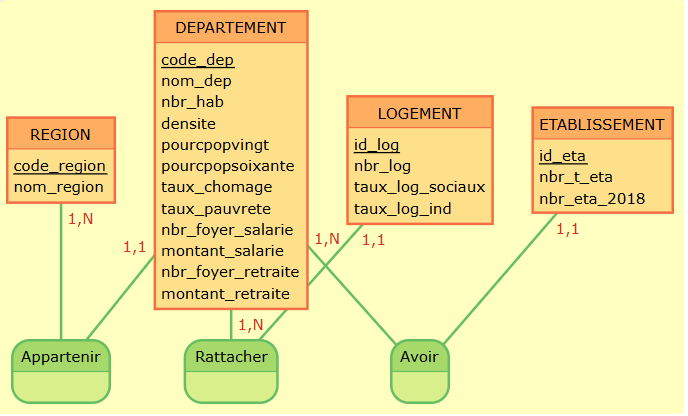
\includegraphics[width=8cm,height=4cm]{Images/MCD.png}
  \caption{MCD.}\label{MCD}
  \end{figure}
\item
  A partir de ce modèle conceptuel(MCD), nous avons crée la version
  manuscrite de notre Modèle Organisationnel de Données(MOD): \medskip
\end{itemize}

DEPARTEMENT (code\_dep, nom\_dep, nbr\_hab, densite, pourcpopvingt,
pourcpopsoixante, taux\_chomage, taux\_pauvrete,nbr\_foyer\_salarie,
montant\_salarie, nbr\_foyer\_retraite, montant\_retraite, code\_region)

\medskip

REGION (code\_region, nom\_region)

\medskip

LOGEMENT (id\_log, nbr\_log, taux\_log\_sociaux, taux\_log\_ind,
code\_dep)

\medskip

ETABLISSEMENT (id\_eta, nbr\_t\_eta, nbr\_eta\_2018, code\_dep)

\medskip

Pour le MOD, on inclut une image réalisée avec le designer de
phpmyadmin, visible sur la Figure\(~\)\ref{MOD} ci-dessous :

\begin{figure}
\centering
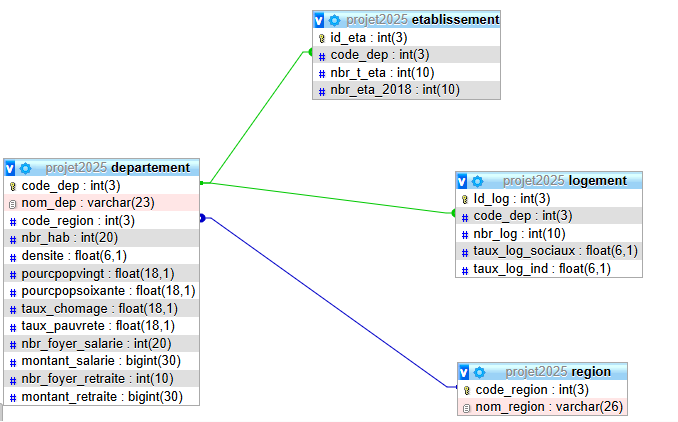
\includegraphics[width=10cm,height=7cm]{Images/MOD.png}
\caption{MOD.}\label{MOD}
\end{figure}

\bigskip

\section{Import des données}\label{import-des-donnuxe9es}

Avant de procéder avec l'importation des données dans PhpMyAdmin, on a
effectué un nettoyage des données. \bigskip

\textbf{Source de données 1}: Nous avons choisi de nous concentrer
uniquement sur les revenus des individus, en distinguant les salariés
des retraités. Toutes les colonnes liées aux impôts et aux autres
données fiscales ont été supprimées, car elles ne relevaient pas de
notre champ d'analyse. Nous avons conservé et renommé uniquement les
colonnes décrivant le département (nom et numéro), ainsi que celles
indiquant le montant des revenus pour les salariés et les retraités.

\medskip

Nous avons filtré la colonne « année » afin de ne conserver que les
données de l'année 2018. Pour la colonne « code\_dep », nous avons
supprimé tous les numéros de département précédés d'un zéro et se
terminant par un zéro, à l'aide d'une fonction Excel. Par ailleurs, nous
avons remplacé les codes des départements de la Corse-du-Sud (2A) et de
la Haute-Corse (2B) par les valeurs 96 et 97,afin d'avoir tous les codes
de départements en entier. Concernant les colonnes retenues, nous avons
nettoyé l'ensemble des données en supprimant les accents, les caractères
spéciaux et les majuscules. Nous avons également simplifié les intitulés
des en-têtes de colonnes. Pour cela, nous avons utilisé la fonction
SUBSTITUTE d'Excel, qui nous a aussi permis de retirer les espaces entre
les chiffres dans les colonnes relatives au nombre de foyers et aux
montants, afin d'assurer une importation correcte des données au format
entier dans MAMP

\bigskip

\textbf{Source de données 2} : Pour cette étude, nous avons retenu les
colonnes relatives au département, à la région d'appartenance, aux
données sur les logements (nombre total de logement, part de logements
sociaux et individuels), ainsi qu'à divers indicateurs socio-économiques
: taux de chômage, taux de pauvreté, densité de population, pourcentage
de la population de moins de 20 ans et de 60 ans et plus.

\medskip

Nous avons trié les départements par ordre alphabétique croissant afin
de faciliter la combinaison des deux jeux de données et de créer une
seule table intitulée « Departement » dans MAMP. Par ailleurs, le
département de Mayotte a été supprimé car il ne figurait pas dans le
second jeu de données et les informations le concernant étaient
incomplètes. Les colonnes retenues ont ensuite été renommées comme suit
: \textbf{code\_dep, nom\_dep, nbr\_foyer\_salarie, montant\_salarie,
nbr\_foyer\_retraite, montant\_retraite,code\_region, nom\_region,
nbr\_hab, densite,pourcpopvingt,pourcpopsoixante, taux\_chomage,
taux\_pauvrete, nbr\_log, taux\_log\_sociaux, taux\_log\_individuel}.

\bigskip

\textbf{Source de données 3} : Pour ce jeu de données, nous avons choisi
d'exclure la colonne relative à la part des établissements culturels
construits en 2018, l'unité de mesure n'étant pas clairement spécifiée.
Il n'était pas possible de déterminer s'il s'agissait d'une valeur
monétaire (en euros, milliers ou millions) ce qui aurait pu fausser
l'interprétation. Les colonnes retenues ont été renommées comme suit:
\textbf{id\_eta, code\_dep, nbr\_t\_eta, nbr\_eta\_2018}.

\bigskip

\section{Requêtes réalisées}\label{requuxeates-ruxe9alisuxe9es}

\textbf{Requête 1}: Lister tous les départements avec leur nom, le
nombre d'habitants et le taux de pauvreté

\begin{Shaded}
\begin{Highlighting}[]
\KeywordTok{SELECT}\NormalTok{ departement.nom\_dep,departement.nbr\_hab ,departement.taux\_pauvrete}
\KeywordTok{from}\NormalTok{ departement}
\end{Highlighting}
\end{Shaded}

\begin{longtable}[]{@{}lrr@{}}
\caption{Displaying records 1 - 10}\tabularnewline
\toprule\noalign{}
nom\_dep & nbr\_hab & taux\_pauvrete \\
\midrule\noalign{}
\endfirsthead
\toprule\noalign{}
nom\_dep & nbr\_hab & taux\_pauvrete \\
\midrule\noalign{}
\endhead
\bottomrule\noalign{}
\endlastfoot
Ain & 643977 & 11 \\
Aisne & 535807 & 19 \\
Allier & 339927 & 16 \\
Alpes-de-Haute-Provence & 161767 & 17 \\
Hautes-Alpes & 141384 & 14 \\
Alpes-Maritimes & 1081455 & 16 \\
Ardeche & 327201 & 15 \\
Ardennes & 273680 & 20 \\
Ariege & 152482 & 19 \\
Aube & 310912 & 16 \\
\end{longtable}

\medskip

\textbf{Requête 2}: Lister les départements dont nom contient le mot «
loire »

\begin{Shaded}
\begin{Highlighting}[]
\KeywordTok{SELECT}\NormalTok{ departement.code\_dep, departement.nom\_dep}
\KeywordTok{from}\NormalTok{ departement}
\KeywordTok{where}\NormalTok{ departement.nom\_dep }\KeywordTok{LIKE} \OtherTok{"\%loire\%"}
\end{Highlighting}
\end{Shaded}

\begin{longtable}[]{@{}rl@{}}
\caption{7 records}\tabularnewline
\toprule\noalign{}
code\_dep & nom\_dep \\
\midrule\noalign{}
\endfirsthead
\toprule\noalign{}
code\_dep & nom\_dep \\
\midrule\noalign{}
\endhead
\bottomrule\noalign{}
\endlastfoot
37 & Indre-et-Loire \\
42 & Loire \\
43 & Haute-Loire \\
44 & Loire-Atlantique \\
45 & Loiret \\
49 & Maine-et-Loire \\
71 & Saone-et-Loire \\
\end{longtable}

\medskip

\textbf{Requête 3}: Lister les départements avec leur densité qui
possèdent un taux de pauvreté inférieur à la moyenne. On affichera les
dix premiers départements qui enregistrent le moins de chômage

\begin{Shaded}
\begin{Highlighting}[]
\KeywordTok{SELECT}\NormalTok{ code\_dep,nom\_dep, densite, taux\_pauvrete}
\KeywordTok{FROM}\NormalTok{ departement}
\KeywordTok{WHERE}\NormalTok{ taux\_pauvrete }\OperatorTok{\textless{}}\NormalTok{ (}\KeywordTok{SELECT} \FunctionTok{AVG}\NormalTok{(taux\_pauvrete) }\KeywordTok{FROM}\NormalTok{ departement)}
\KeywordTok{ORDER} \KeywordTok{BY}\NormalTok{ taux\_pauvrete }
\KeywordTok{LIMIT} \DecValTok{10}\NormalTok{;}
\end{Highlighting}
\end{Shaded}

\begin{longtable}[]{@{}rlrr@{}}
\caption{Displaying records 1 - 10}\tabularnewline
\toprule\noalign{}
code\_dep & nom\_dep & densite & taux\_pauvrete \\
\midrule\noalign{}
\endfirsthead
\toprule\noalign{}
code\_dep & nom\_dep & densite & taux\_pauvrete \\
\midrule\noalign{}
\endhead
\bottomrule\noalign{}
\endlastfoot
74 & Haute-Savoie & 186 & 9.0 \\
85 & Vendee & 101 & 10.0 \\
78 & Yvelines & 628 & 10.0 \\
44 & Loire-Atlantique & 215 & 10.0 \\
73 & Savoie & 72 & 10.0 \\
1 & Ain & 112 & 11.0 \\
29 & Finistere & 135 & 11.0 \\
35 & Ille-et-Vilaine & 157 & 11.0 \\
56 & Morbihan & 110 & 11.0 \\
21 & Cote-d'Or & 61 & 11.5 \\
\end{longtable}

\medskip

\textbf{Requête 4} : Lister les départements avec leur densité qui
possèdent un taux de chômage inférieur à la moyenne. On affichera les
dix premiers départements qui enregistrent le moins de chômage

\begin{Shaded}
\begin{Highlighting}[]
\KeywordTok{SELECT}\NormalTok{ code\_dep,nom\_dep, densite, taux\_chomage}
\KeywordTok{FROM}\NormalTok{ departement}
\KeywordTok{WHERE}\NormalTok{ taux\_chomage }\OperatorTok{\textless{}}\NormalTok{ (}\KeywordTok{SELECT} \FunctionTok{AVG}\NormalTok{(taux\_chomage) }\KeywordTok{FROM}\NormalTok{ departement)}
\KeywordTok{ORDER} \KeywordTok{BY}\NormalTok{ taux\_chomage}
\KeywordTok{LIMIT} \DecValTok{10}\NormalTok{;}
\end{Highlighting}
\end{Shaded}

\begin{longtable}[]{@{}rlrr@{}}
\caption{Displaying records 1 - 10}\tabularnewline
\toprule\noalign{}
code\_dep & nom\_dep & densite & taux\_chomage \\
\midrule\noalign{}
\endfirsthead
\toprule\noalign{}
code\_dep & nom\_dep & densite & taux\_chomage \\
\midrule\noalign{}
\endhead
\bottomrule\noalign{}
\endlastfoot
15 & Cantal & 25 & 5.0 \\
44 & Loire-Atlantique & 215 & 5.5 \\
96 & Corse-du-Sud & 40 & 5.8 \\
21 & Cote-d'Or & 61 & 5.8 \\
1 & Ain & 112 & 6.0 \\
53 & Mayenne & 59 & 6.0 \\
74 & Haute-Savoie & 186 & 6.0 \\
39 & Jura & 52 & 6.0 \\
92 & Hauts-de-Seine & 9122 & 6.0 \\
48 & Lozere & 15 & 6.0 \\
\end{longtable}

\medskip

Les requêtes 3 et 4 fournissent des éléments sur la situation économique
des départements, notamment à travers les taux de chômage et de
pauvreté. Bien que ces indicateurs soient importants, ils ne suffisent
pas à eux seuls à déterminer dans quels départements l'on vit le mieux.
Les résultats montrent que les départements ayant les taux de chômage
les plus faibles ne sont pas nécessairement ceux où la pauvreté est la
moins présente. Certains départements, comme la Côte-d'Or, la
Haute-Savoie et l'Ain, présentent toutefois des taux faibles pour ces
deux indicateurs.

L'information relative à la densité de population permet également
d'apprécier si ces départements sont fortement peuplés ou non. On
observe que, mis à part Hauts-Savoie et Yvelines, les départements
concernés sont peu ou moyennement peuplés.

\medskip

\textbf{Requête 5} : Lister les dix départements français qui présentent
la densité de population la plus élevée.

\begin{Shaded}
\begin{Highlighting}[]
\KeywordTok{SELECT}\NormalTok{ departement.code\_dep,departement.nom\_dep,departement.densite}
\KeywordTok{FROM}\NormalTok{ departement}
\KeywordTok{ORDER} \KeywordTok{BY}\NormalTok{ departement.densite }\KeywordTok{DESC}
\KeywordTok{LIMIT} \DecValTok{10}\NormalTok{;}
\end{Highlighting}
\end{Shaded}

\begin{longtable}[]{@{}rlr@{}}
\caption{Displaying records 1 - 10}\tabularnewline
\toprule\noalign{}
code\_dep & nom\_dep & densite \\
\midrule\noalign{}
\endfirsthead
\toprule\noalign{}
code\_dep & nom\_dep & densite \\
\midrule\noalign{}
\endhead
\bottomrule\noalign{}
\endlastfoot
75 & Paris & 20780 \\
92 & Hauts-de-Seine & 9122 \\
93 & Seine-Saint-Denis & 6900 \\
94 & Val-de-Marne & 5762 \\
95 & Val-d'Oise & 997 \\
91 & Essonne & 721 \\
78 & Yvelines & 628 \\
69 & Rhone & 573 \\
59 & Nord & 455 \\
13 & Bouches-du-Rhone & 400 \\
\end{longtable}

\medskip

\textbf{Requête 6} : Lister départements avec le montant des revenues
des salariés par ordre décroissant.

\begin{Shaded}
\begin{Highlighting}[]
\KeywordTok{SELECT}\NormalTok{ departement.code\_dep,departement.nom\_dep,departement.montant\_salarie}
\KeywordTok{FROM}\NormalTok{ departement}
\KeywordTok{ORDER} \KeywordTok{BY}\NormalTok{ departement.montant\_salarie }\KeywordTok{DESC}
\end{Highlighting}
\end{Shaded}

\begin{longtable}[]{@{}rlr@{}}
\caption{Displaying records 1 - 10}\tabularnewline
\toprule\noalign{}
code\_dep & nom\_dep & montant\_salarie \\
\midrule\noalign{}
\endfirsthead
\toprule\noalign{}
code\_dep & nom\_dep & montant\_salarie \\
\midrule\noalign{}
\endhead
\bottomrule\noalign{}
\endlastfoot
75 & Paris & 43166479210 \\
92 & Hauts-de-Seine & 29829489811 \\
59 & Nord & 24599283600 \\
78 & Yvelines & 23132191421 \\
69 & Rhone & 22296487843 \\
13 & Bouches-du-Rhone & 21327075837 \\
94 & Val-de-Marne & 18572641397 \\
77 & Seine-et-Marne & 17555206317 \\
33 & Gironde & 17414630484 \\
91 & Essonne & 17210174957 \\
\end{longtable}

\medskip

\textbf{Requête 7} : Lister les dix départements les plus peuplés et le
revenu des salariés correspondant .On donnera aussi le nombre de
logements de ces départements

\begin{Shaded}
\begin{Highlighting}[]
\KeywordTok{SELECT}\NormalTok{ d.nom\_dep, d.nbr\_hab, d.montant\_salarie, l.nbr\_log}
\KeywordTok{FROM}\NormalTok{ departement d}
\KeywordTok{JOIN}\NormalTok{ logement l }\KeywordTok{ON}\NormalTok{ d.code\_dep }\OperatorTok{=}\NormalTok{ l.code\_dep}
\KeywordTok{ORDER} \KeywordTok{BY}\NormalTok{ d.nbr\_hab }\KeywordTok{DESC}
\KeywordTok{LIMIT} \DecValTok{10}\NormalTok{;}
\end{Highlighting}
\end{Shaded}

\begin{longtable}[]{@{}lrrr@{}}
\caption{Displaying records 1 - 10}\tabularnewline
\toprule\noalign{}
nom\_dep & nbr\_hab & montant\_salarie & nbr\_log \\
\midrule\noalign{}
\endfirsthead
\toprule\noalign{}
nom\_dep & nbr\_hab & montant\_salarie & nbr\_log \\
\midrule\noalign{}
\endhead
\bottomrule\noalign{}
\endlastfoot
Nord & 2612189 & 24599283600 & 1194450 \\
Paris & 2181866 & 43166479210 & 1366438 \\
Bouches-du-Rhone & 2035414 & 21327075837 & 1000230 \\
Rhone & 1860112 & 22296487843 & 890850 \\
Seine-Saint-Denis & 1628410 & 15920780899 & 652707 \\
Hauts-de-Seine & 1605502 & 29829489811 & 789809 \\
Gironde & 1590570 & 17414630484 & 828907 \\
Pas-de-Calais & 1474943 & 12551458646 & 703500 \\
Loire-Atlantique & 1462506 & 15395217771 & 776207 \\
Yvelines & 1434980 & 23132191421 & 621026 \\
\end{longtable}

\medskip

L'objectif de cette requête est d'examiner si les départements les plus
peuplés c'est-à-dire avec le plus grand nombre d'habitants présentent
également un revenu moyen plus élevé ainsi qu'une proportion plus
importante de logements que les autres.

Les résultats montrent que le nombre d'habitants n'est pas
nécessairement proportionnel au revenu moyen des salariés ni au nombre
de logements par département. Par exemple, le département du Nord est
plus peuplé que Paris, mais cette dernière compte davantage de logements
et affiche un revenu moyen des salariés plus élevé.

\medskip

\textbf{Requête 8} : Lister les départements qui possèdent le plus
d'établissements culturels

\begin{Shaded}
\begin{Highlighting}[]
\KeywordTok{SELECT}\NormalTok{ d.code\_dep, d.nom\_dep, e.nbr\_t\_eta}
\KeywordTok{FROM}\NormalTok{ departement d, etablissement e}
\KeywordTok{WHERE}\NormalTok{ d.code\_dep}\OperatorTok{=}\NormalTok{e.code\_dep}
\KeywordTok{ORDER} \KeywordTok{BY}\NormalTok{ nbr\_t\_eta }\KeywordTok{DESC}
\KeywordTok{LIMIT} \DecValTok{10}\NormalTok{;}
\end{Highlighting}
\end{Shaded}

\begin{longtable}[]{@{}rlr@{}}
\caption{Displaying records 1 - 10}\tabularnewline
\toprule\noalign{}
code\_dep & nom\_dep & nbr\_t\_eta \\
\midrule\noalign{}
\endfirsthead
\toprule\noalign{}
code\_dep & nom\_dep & nbr\_t\_eta \\
\midrule\noalign{}
\endhead
\bottomrule\noalign{}
\endlastfoot
75 & Paris & 182079 \\
13 & Bouches-du-Rhone & 74510 \\
69 & Rhone & 72720 \\
59 & Nord & 68081 \\
33 & Gironde & 59594 \\
92 & Hauts-de-Seine & 57534 \\
6 & Alpes-Maritimes & 49039 \\
31 & Haute-Garonne & 46972 \\
93 & Seine-Saint-Denis & 46637 \\
44 & Loire-Atlantique & 45318 \\
\end{longtable}

\medskip

Avec cette requête et la 5, on a pu observer que les départements ayant
le plus grand nombre d'établissements sont, pour la plupart, ceux ayant
la densité la plus élevée.

\medskip

\textbf{Requête 9}: Afficher le nombre d'établissement total par region
et le nom de la region

\begin{Shaded}
\begin{Highlighting}[]
\KeywordTok{SELECT}\NormalTok{ r.nom\_region, }\FunctionTok{SUM}\NormalTok{(e.nbr\_t\_eta) }\KeywordTok{AS}\NormalTok{ total\_etablissements}
\KeywordTok{FROM}\NormalTok{ region r}
\KeywordTok{JOIN}\NormalTok{ departement d }\KeywordTok{ON}\NormalTok{ r.code\_region }\OperatorTok{=}\NormalTok{ d.code\_region}
\KeywordTok{JOIN}\NormalTok{ etablissement e }\KeywordTok{ON}\NormalTok{ d.code\_dep }\OperatorTok{=}\NormalTok{ e.code\_dep}
\KeywordTok{GROUP} \KeywordTok{BY}\NormalTok{ r.nom\_region}
\KeywordTok{ORDER} \KeywordTok{BY}\NormalTok{ total\_etablissements }\KeywordTok{DESC}\NormalTok{;}
\end{Highlighting}
\end{Shaded}

\begin{longtable}[]{@{}lr@{}}
\caption{Displaying records 1 - 10}\tabularnewline
\toprule\noalign{}
nom\_region & total\_etablissements \\
\midrule\noalign{}
\endfirsthead
\toprule\noalign{}
nom\_region & total\_etablissements \\
\midrule\noalign{}
\endhead
\bottomrule\noalign{}
\endlastfoot
ile-de-france & 470619 \\
auvergne-rhone-alpes & 287141 \\
nouvelle-aquitaine & 216351 \\
occitanie & 212823 \\
provence-alpes-cote d'azur & 202450 \\
grand est & 174773 \\
hauts-de-france & 158079 \\
pays de la loire & 120335 \\
bretagne & 109839 \\
normandie & 104304 \\
\end{longtable}

\medskip

Cette requête donne une vision globale de l'offre d'infrastructures dans
chaque région, ce qui peut être un critère de qualité de vie. Les
régions avec plus d'établissements culturels peuvent offrir des
conditions de vie plus favorables en termes d'accès à la culture.

Nous pouvons observer que la région Île-de-France regroupe les
départements les plus peuplés en termes de densité, ce qui en fait la
région avec le plus grand nombre d'infrastructures culturelles.

\medskip

\textbf{Requête 10} : Lister dix départements avec les taux de logements
sociaux les plus faibles et les revenus des salariés correspondants

\begin{Shaded}
\begin{Highlighting}[]
\KeywordTok{SELECT}\NormalTok{ d.code\_dep,d.nom\_dep, l.taux\_log\_sociaux ,d.montant\_salarie}
\KeywordTok{FROM}\NormalTok{ departement d}
\KeywordTok{JOIN}\NormalTok{ logement l }\KeywordTok{ON}\NormalTok{ d.code\_dep }\OperatorTok{=}\NormalTok{ l.code\_dep}
\KeywordTok{ORDER} \KeywordTok{BY}\NormalTok{ l.taux\_log\_sociaux }\KeywordTok{ASC}
\KeywordTok{LIMIT} \DecValTok{10}\NormalTok{;}
\end{Highlighting}
\end{Shaded}

\begin{longtable}[]{@{}rlrr@{}}
\caption{Displaying records 1 - 10}\tabularnewline
\toprule\noalign{}
code\_dep & nom\_dep & taux\_log\_sociaux & montant\_salarie \\
\midrule\noalign{}
\endfirsthead
\toprule\noalign{}
code\_dep & nom\_dep & taux\_log\_sociaux & montant\_salarie \\
\midrule\noalign{}
\endhead
\bottomrule\noalign{}
\endlastfoot
9 & Ariege & 5 & 1157893556 \\
12 & Aveyron & 6 & 2200576943 \\
32 & Gers & 6 & 1575089365 \\
46 & Lot & 6 & 1335539711 \\
24 & Dordogne & 7 & 3143389291 \\
40 & Landes & 7 & 3686812472 \\
47 & Lot-et-Garonne & 7 & 2667465826 \\
48 & Lozere & 8 & 586070966 \\
19 & Correze & 8 & 2018605916 \\
43 & Haute-Loire & 8 & 1928086321 \\
\end{longtable}

\medskip

Cette requête nous permet de voir que les départements présentant les
taux de logements sociaux les plus faibles ne sont pas forcément ceux
ayant les revenus les plus élevés, comme on pourrait le croire. Au
contraire, par exemple, des départements comme la Lozère, l'Ariège et le
Lot sont des départements ayant à la fois les revenus salariaux les plus
bas et les taux de logements sociaux les plus faibles.

\chapter{Matériel et Méthodes}\label{matuxe9riel-et-muxe9thodes}

\section{Logiciels}\label{logiciels}

Pour faciliter les échanges tout au long du projet, nous avons utilisé
le logiciel Google Docs avec un dossier partagé, dans lequel chacune
avançait sur sa partie.

\medskip

Pour travailler et communiquer en temps réel, nous avons également
utilisé l'application WhatsApp ainsi que les adresses mail de
l'université afin de nous transmettre, à tour de rôle, chaque nouvelle
modification apportée.

\medskip

Le logiciel Excel nous a permis de supprimer les colonnes inutiles, de
nettoyer les données comme évoqué dans la partie sur l'importation des
données et de créer différentes feuilles correspondant aux tables.

\medskip

Grâce à l'outil open-source MOCODO, nous avons pu créer le Modèle
Conceptuel de Données(MCD). Et ensuite avec l'application MAMP, via
l'interface PhpMyAdmin, nous avons créer le Modèle Organisationnel de
Données (MOD) et manipuler nos données pour réaliser les requêtes
nécessaires.

\medskip

Nous avons ensuite utilisé le logiciel R, à travers son interface
RStudio, pour effectuer des analyses statistiques, produire des
graphiques, établir une connexion directe avec notre base de données, et
générer un rapport complet au format PDF à l'aide de R Markdown.

\medskip

Enfin, nous avons eu recours à l'outil d'intelligence artificielle
générative ChatGPT pour la correction orthographique ainsi que pour
l'amélioration rédactionnelle de l'ensemble du rapport.Tout en précisant
qu'on ne lui a pas demandé de nous générer directement du texte, ce sont
nos propres textes qu'il a juste corrigé.

\medskip

Les analyses ont été réalisées sur un ordinateur fonctionnant sous
Windows 11, équipé d'un processeur Intel Core i7-1065G7 cadencé à 1,30
GHz, de 32 Go de mémoire vive, d'un stockage de 512 Go et d'une carte
graphique Intel Iris Plus Graphics.

\section{Modélisation statistique}\label{moduxe9lisation-statistique}

Pour les analyses des relations entre nos variables nous avons utilisé
le logiciel R Markdown.

\medskip

Nous avons utilisé deux outils fondamentaux: le test de corrélation de
Pearson et l'analyse de variance (ANOVA).

\bigskip

\subsection{Le test de corrélation de
Pearson}\label{le-test-de-corruxe9lation-de-pearson}

Ce test évalue l'intensité et le signe d'une relation linéaire entre
deux variables quantitatives. \medskip

Pour son utilisation dans R on a utilisé la fonction cor() pour le
simple calcul et cor.test() pour effectuer le test de corrélation.
\medskip

\begin{center} 

$$
r =\frac {{Cov}(X,Y)} {\sigma(X) \cdot \sigma (Y)}
$$

\end{center}
\medskip

\subsection{Analyse de la variance}\label{analyse-de-la-variance}

L'ANOVA est utilisé pour comparer les moyennes de plusieurs groupes et
se base sur la décomposition de la variance totale en ses deux
composantes: la variance INTER et la variance INTRA. \medskip

La statistique de test pour le test d'ANOVA peut s'écrire:

\[
\frac {INTER} {INTRA}  (n-K)
\] \(n=\) effectifs et \(K=\) nombre de groupes

\medskip

Pour effectuer le test d'ANOVA sur R on a utilisé la fonction aov().

\bigskip

\chapter{Analyse Exploratoire des
Données}\label{analyse-exploratoire-des-donnuxe9es}

Après avoir importé les fichiers ( Departement.csv, Etablissement.csv,
Logement.csv ) contenant nos données, on a pu coder les types des
variables de notre jeu de données ( codes en annexe). Avec ceci on a
créé des data frames pour mieux traiter les données.

\bigskip

\section{Import des fichiers csv utiles aux analyses
statistiques}\label{import-des-fichiers-csv-utiles-aux-analyses-statistiques}

Voici la nature des variables utilisées:

\medskip

\begin{itemize}
\tightlist
\item
  montant\_salarie : variable quantitative continue
\end{itemize}

\medskip

\begin{itemize}
\tightlist
\item
  taux\_chomage : variable quantitative continue
\end{itemize}

\medskip

\begin{itemize}
\tightlist
\item
  taux\_chomage : variable quantitative continue
\end{itemize}

\medskip

\begin{itemize}
\tightlist
\item
  taux\_log\_sociax : variable quantitative continue
\end{itemize}

\medskip

\begin{itemize}
\tightlist
\item
  nbr\_t\_eta : variable quantitative discrète
\end{itemize}

\bigskip

\section{Analyses univariées}\label{analyses-univariuxe9es}

On considère d'abord la variable \textbf{nombre d'habitants par
départements}. Pour mieux la visualiser la représente à l'aide d'un
histogramme.

\begin{center}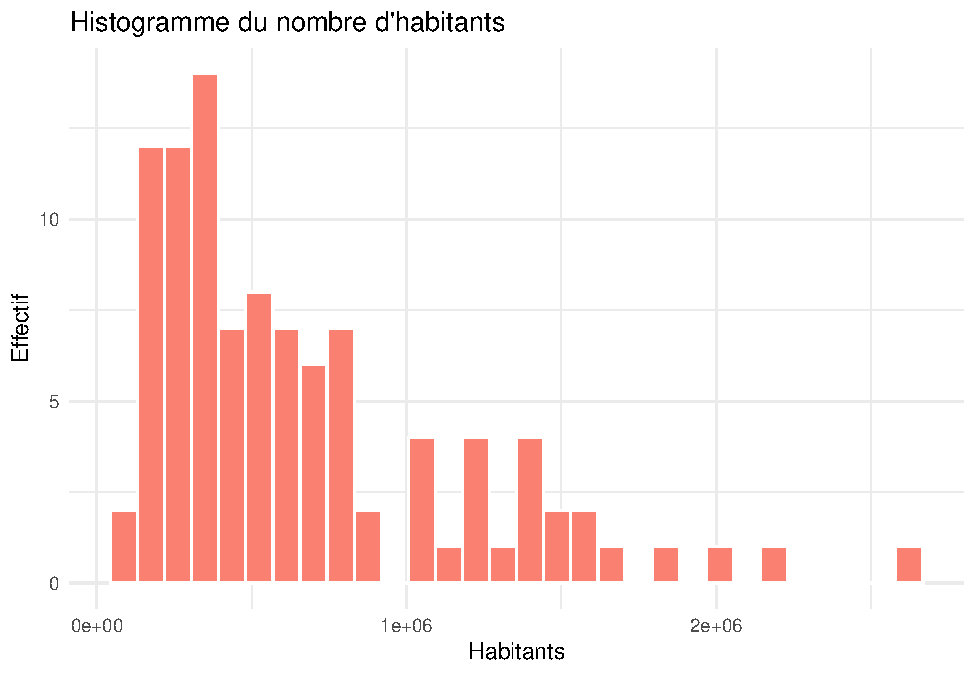
\includegraphics[width=12cm]{GroupReportTemplate-2_files/figure-latex/unnamed-chunk-15-1} \end{center}

\normalsize

On remarque une grande disparité dans la répartition du nombre
d'habitants par département, comme on peut le voir avec certains
départements très peuplés et d'autres n'enregistrant que peu
d'habitants.

\medskip

On calcule la moyenne globale: \medskip

\begin{verbatim}
## [1] 668516.3
\end{verbatim}

\medskip

On calcule la mediane globale:

\begin{verbatim}
## [1] 534985.5
\end{verbatim}

\bigskip

Maintenant on va considérer la variable \textbf{nombre de logements par
départements}. Comme pour la variable précédente on va la représenter
grâce à un histogramme. \medskip

\begin{center}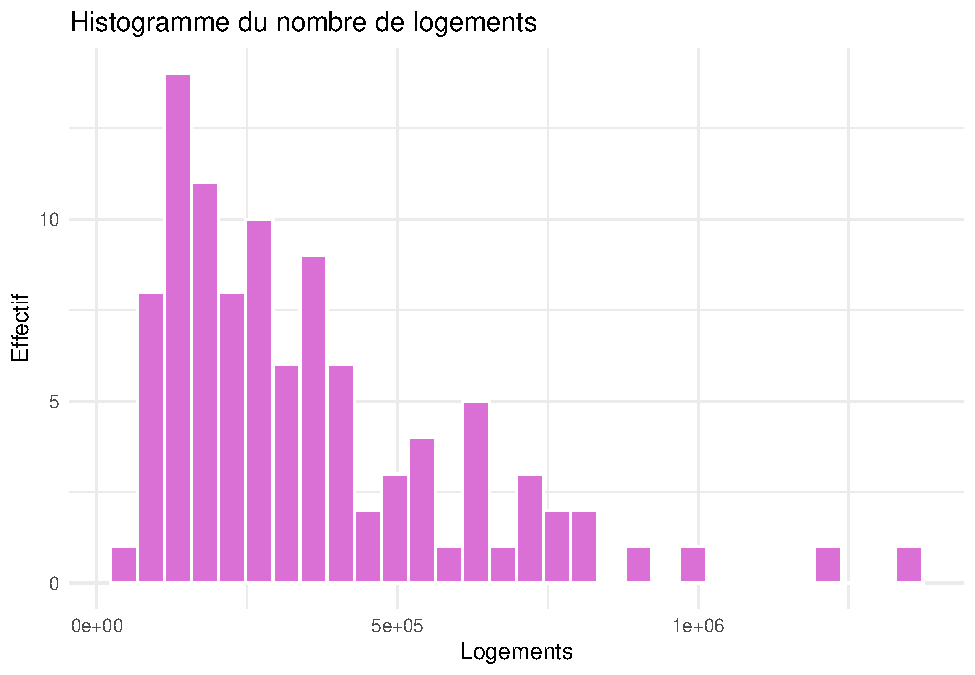
\includegraphics[width=12cm]{GroupReportTemplate-2_files/figure-latex/unnamed-chunk-18-1} \end{center}
\medskip

On constate une grande disparité dans la répartition du nombre de
logements par département, comme on peut le voir avec certains
départements ayant de nombreux logements et d'autres n'enregistrant que
peu de logements.

\bigskip

Selon notre hypothèse, les disparités importantes pourraient être dû au
fait qu'un département plus peuplé ait plus de logements qu'un
département moins peuplé. On va vérifier cela dans la partie suivante de
l'analyse bivariée.

\bigskip

\section{Analyses bivariées}\label{analyses-bivariuxe9es}

On commence par analyser la relation entre les \textbf{variables montant
salaire et le taux de chômage}. Afin de mieux visualiser un lien
éventuel entre les variables, on représente le nuage de points des
variables montant\_salaire et taux\_chomage: \medskip 

\begin{center}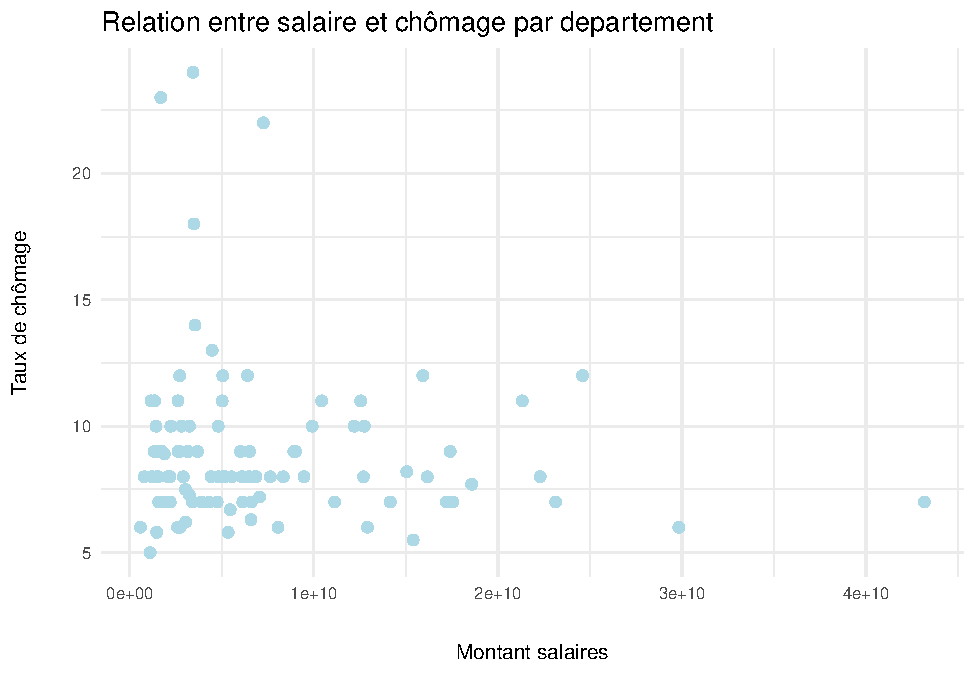
\includegraphics[width=12cm]{GroupReportTemplate-2_files/figure-latex/unnamed-chunk-19-1} \end{center}
\medskip

On observe un nuage de points très dispersé, avec cinq points
particulièrement éloignés des autres. Il ne semble pas y avoir de lien
entre le montant des salaires générés par département et le taux de
chômage. \medskip 

A partir du nuage de points on peut supposer que entre les deux
variables il n'y a pas de liaison, on calcule donc le coefficient de
corrélation: \medskip 

Après le calcul on obtient le coefficient de corrélation:

\medskip

\begin{verbatim}
## [1] -0.1009249
\end{verbatim}

\medskip

Ce résultat montre une corrélation inverse faible entre les deux
variables. Pour approfondir notre analyse, on passe au test de
corrélation entre les deux variables.

\medskip

\textbf{Hypothèse H}: les variables montant\_salaire et taux\_chomage ne
sont pas corrélées On procède avec le test à l'aide de la fonction
cor.test sur R, qui nous fournit tous les détailles:

\medskip

\begin{verbatim}
## 
##  Pearson's product-moment correlation
## 
## data:  departement$montant_salarie and departement$taux_chomage
## t = -1.0042, df = 98, p-value = 0.3177
## alternative hypothesis: true correlation is not equal to 0
## 95 percent confidence interval:
##  -0.29156323  0.09742451
## sample estimates:
##        cor 
## -0.1009249
\end{verbatim}

\medskip

Le résultat nous indique une relation linéaire non significative entre
les variables montant salaire et taux chômage avec un coefficient de
corrélation r = -0.10.

\medskip

La co-valeure 0.3177 est inférieure à 0.05, cela implique qu' avec un
niveau de confiance de 95\%, on ne peut rejeter l'hypothèse H.

\medskip

Il n'existe donc aucune association linéaire significative entre le
montant des salaires par département et le taux de chômage. On en déduit
que les salaires n'ont pas d'influence sur le taux de chômage.

\bigskip

Il est aussi intéressant de voir si les variables
\textbf{montant\_salaire et taux\_pauvrete} sont corrélées. Voici le
nuage des points des deux variables:

\begin{center}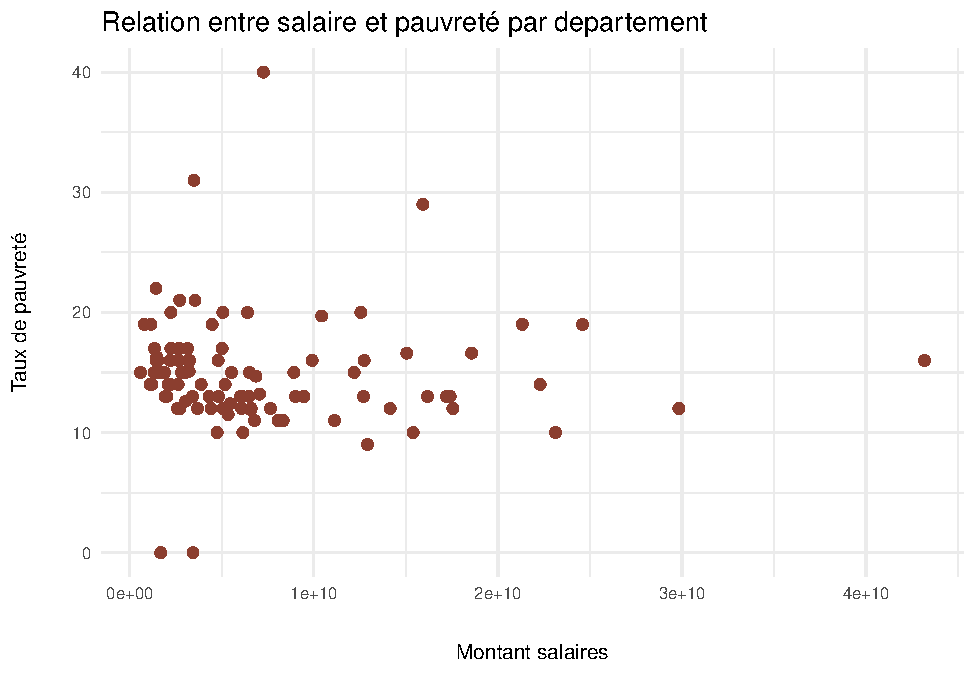
\includegraphics[width=12cm]{GroupReportTemplate-2_files/figure-latex/unnamed-chunk-22-1} \end{center}

\medskip

On observe un nuage de points un peu plus condensé, avec également cinq
points qui restent quelque peu isolés par rapport aux autres.

\medskip

A partir du nuage des points il semble qu'il n'y ait pas de lien entre
le montant des salaires générés par département et le taux de pauvreté
dans ces départements.

\medskip

On calcule donc le coefficient de corrélation:

\medskip

\begin{verbatim}
## [1] -0.01538043
\end{verbatim}

\medskip

Ce résultat montre une corrélation inverse très faible entre les deux
variables.

\medskip

Comme avant on procède au test de corrélation entre ces variables:

\medskip

\textbf{Hypothèse H}: les variables montant\_salaire et taux\_pauvrete
ne sont pas corrélés.

\medskip

Voici les résultats du test en détail:

\medskip

\begin{verbatim}
## 
##  Pearson's product-moment correlation
## 
## data:  departement$montant_salarie and departement$taux_pauvrete
## t = -0.15228, df = 98, p-value = 0.8793
## alternative hypothesis: true correlation is not equal to 0
## 95 percent confidence interval:
##  -0.2111606  0.1815863
## sample estimates:
##         cor 
## -0.01538043
\end{verbatim}

\medskip

On a bien confirmé que il y a une relation linéaire non significative
entre les variables montant\_salaire et taux\_pauvrete, avec un
coefficient de corrélation r=-0.015 \medskip

La p-valeure de 0.8793 est largement supérieure à 0.05, cela implique
qu'avec un niveau de confiance de 95\%, on ne peut pas rejeter
l'hypothèse H. \medskip

Il n'existe donc aucune association linéaire significative entre le
montant des salaires par département et le taux de pauvreté. On en
déduit que les salaires n'ont pas d'influence sur le taux de pauvreté.

\bigskip

On passe finalement à l'analyse des relations entre les variables
\textbf{nbr\_t\_eta et t\_log\_soc}: Voici le nuage des points: \medskip

\begin{center}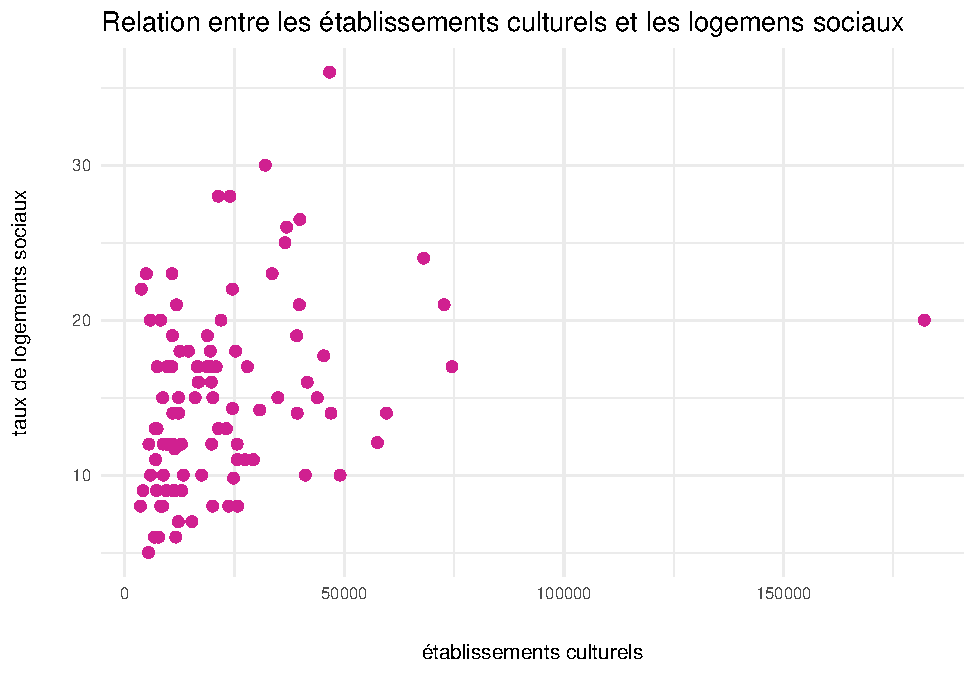
\includegraphics[width=12cm]{GroupReportTemplate-2_files/figure-latex/unnamed-chunk-25-1} \end{center}
\medskip

On observe un nuage de points légèrement éparpillé, avec un point
atypique particulièrement éloigné des autres. On pourrait supposer
l'existence d'un lien positif faible entre les deux variables.
Toutefois, il est également possible qu'il n'existe aucun lien entre le
nombre d'établissements culturels et le taux de logements sociaux dans
un département.

\medskip

Pour vérifier cela on calcule le coefficient de corrélation:

\medskip

\begin{verbatim}
## [1] 0.3083597
\end{verbatim}

\medskip

Le résultat nous montre une corrélation faible positive entre les deux
variables.

\medskip

On passe au test de corrélation pour mieux analyser ce lien.

\medskip

\textbf{Hypothèse H}: les variables nombre d'établissements culturels et
taux de logements sociaux ne sont pas corrélées.

\medskip

On procède avec le test avec la fonction cor.test pour plus de détails:

\medskip

\begin{verbatim}
## 
##  Pearson's product-moment correlation
## 
## data:  etablissement$nbr_t_eta and logement$t_log_soc
## t = 3.209, df = 98, p-value = 0.001801
## alternative hypothesis: true correlation is not equal to 0
## 95 percent confidence interval:
##  0.1191588 0.4759507
## sample estimates:
##       cor 
## 0.3083597
\end{verbatim}

\medskip

Le résultat nous suggère une relation linéaire positive entre entre les
variables nombre d'établissements culturels et taux de logements
sociaux, avec un coefficient de corrélation r = 0.31.

\medskip

La p-valeur de 0.0018 est bien inférieure à 0.05, ce qui implique
qu'avec un niveau de confiance de 95\%, on peut rejeter l'hypothèse H et
conclure qu'il existe une corrélation significative entre les deux
variables.

\medskip

Il existe donc une association linéaire positive entre le nombre
d'établissements culturels et le taux de logements sociaux par
département. Les résultats suggèrent que les départements ayant
davantage d'établissements culturels tendent également à avoir un taux
de logements sociaux plus élevé.

\bigskip

\section{Test d'ANOVA}\label{test-danova}

Nous souhaitons étudier si le revenu par classe a un effet significatif
sur le nombre d'établissements culturels par département. Pour cela nous
avons réalisé un test d'ANOVA (analyse de variance à un facteur).

\medskip

Les données concernant la variable montant\_salaire ont été classées en
quatre catégories (selon les quartiles) afin de les transformer en une
variable qualitative ordinale catégorie de revenu avec 4 modalités:
\textbf{faible, moyen-faible, moyen-élevé et élevé}.

\medskip

L'objectif de cette analyse est de déterminer si le niveau de revenu
d'un département (catégorie de revenu) a un impact significatif sur le
nombre d'établissements culturels présents sur son territoire.

\medskip

Nous utilisons donc un test d'ANOVA à un facteur pour répondre à cette
question.

\medskip

\textbf{Hypothèse}: Les revenus par classe n'ont pas d'impact sur la
distribution du nombre total d'établissements culturels dans chaque
département.

\medskip

Nous avons appliqué le test d'ANOVA pour comparer les moyennes du nombre
d'établissements culturels entre ces groupes:

\bigskip

\begin{verbatim}
##                  Df    Sum Sq   Mean Sq F value   Pr(>F)    
## categorie_revenu  3 2.626e+10 8.752e+09   35.94 1.17e-15 ***
## Residuals        96 2.338e+10 2.435e+08                     
## ---
## Signif. codes:  0 '***' 0.001 '**' 0.01 '*' 0.05 '.' 0.1 ' ' 1
\end{verbatim}

\medskip

La statistique de test F est calculée comme le rapport de la variance
inter-groupes a la variance intra-groupes. ici F=234.4 qui indique une
variabilité entre groupes supérieure à celle à l'intérieur des groupes.
En plus la p-valeur associée est extrêmement faible
(\(1.17 × 10^-{15}\)), bien inférieure au seuil de 0.05.

\medskip

Puisque la p-valeur est très inférieure à 0.05, on rejette l'hypothèse.
On peut donc dire qu'il existe une difference tres significative du
nombre moyen d'établissement culturels selon la catégorie de revenu.

\medskip

Le revenu a donc un effet et sur le nombre d'établissements culturels.

\bigskip

Visualisons avec un box-plot le nombre d'établissements culturels par
catégorie de revenu.

\begin{figure}

{\centering 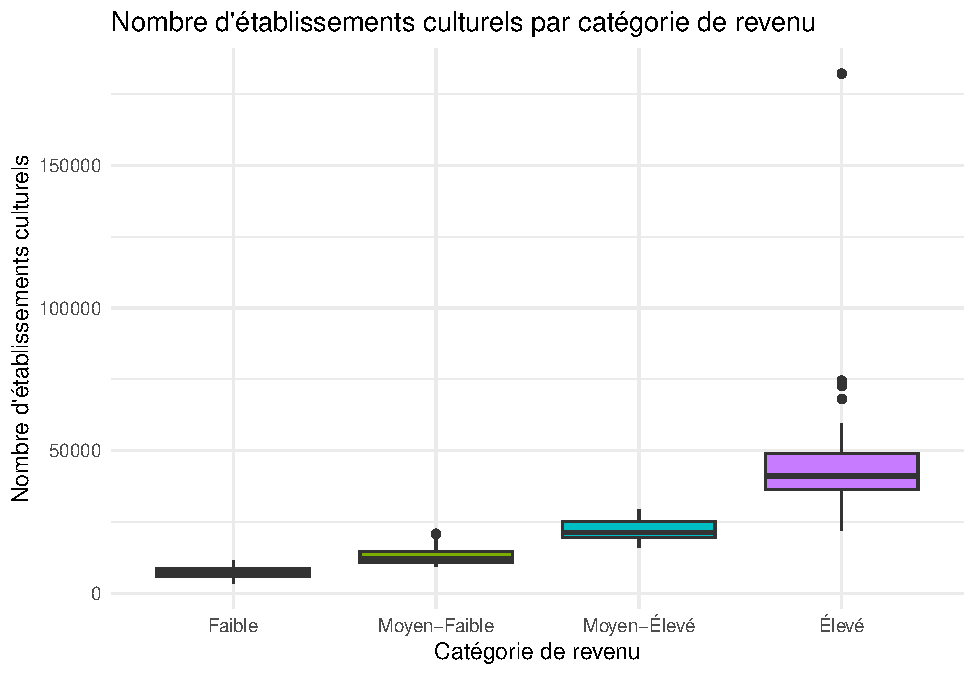
\includegraphics[width=12cm]{GroupReportTemplate-2_files/figure-latex/unnamed-chunk-29-1} 

}

\caption{Nombre d'établissements culturels par catégorie de revenu}\label{fig:unnamed-chunk-29}
\end{figure}

\medskip

Le boxplot du nombre d'établissements culturels par catégorie de revenu
montre visuellement que: le nombre d'établissements augmente nettement
avec la catégorie de revenu.

\medskip

La médiane et la dispersion sont plus élevées dans les groupes à revenu
élevé.

\bigskip

En conclusion, le test d'ANOVA montre que \textbf{le revenu moyen d'un
département à un effet significatif sur le nombre d'établissements
culturels}.

\chapter{Discussion}\label{discussion}

Notre analyse a relevé une absence de corrélation significative entre le
montant des salaires et le taux de chômage, ainsi qu'entre le montant
des salaires et le taux de pauvreté. Ces résultats contredisent
l'hypothèse selon laquelle les départements aux revenus plus élevés
offraient nécessairement de meilleures conditions de vie. En effet,
certains départements comme Paris ou les Hauts-de-Seine présentent des
revenus parmi les plus élevés, mais cela ne se traduit pas
automatiquement par des taux de chômage ou de pauvreté plus faibles.

\medskip

L'absence de corrélation suggère que d'autres facteurs influencent la
qualité de vie dans les départements. Par exemple, le coût de la vie ou
le prix de l'immobilier,etc.

\medskip

En revanche, le test d'ANOVA a démontré une relation significative entre
le niveau de revenu d'un département et le nombre d'établissements
culturels. Le boxplot illustre clairement que les départements à revenus
élevés disposent en moyenne davantage d'établissements culturels. Cette
partie de notre hypothèse initiale se trouve donc confirmée: les
départements économiquement plus favorisés offrent effectivement un
accès plus important à la culture.

\medskip

Cependant cette relation mérite d'être nuancée.La présence
d'infrastructures culturelles pourrait être davantage liée à la densité
de la population qu'au revenu en lui- même. Nos requêtes SQL ont montré
que les départements avec le plus d'établissements culturels
correspondent en grand partie à ceux ayant les densités de population
les plus élevées.

\medskip

Contrairement à notre hypothèse initiale, l'analyse montre une
corrélation positive significative entre le nombre d'établissements
culturels et le taux de logements sociaux. Ainsi les départements
disposant de nombreuses infrastructures culturelles tendent également à
avoir une proportion plus importante de logements sociaux, ce qui va à
l'encontre de l'idée que les départements offrant les meilleures
conditions de vie auraient moins de logements sociaux.

\bigskip

\chapter{Conclusion}\label{conclusion}

Cette étude a permis d'explorer la question des meilleures conditions de
vie dans les départements français, en les liant à des critères tels que
les revenus moyens, l'accès aux infrastructures culturelles, et la
proportion de logements sociaux. Les résultats ont remis en cause l'idée
selon laquelle les départements avec les revenus les plus élevés sont
automatiquement ceux offrant les meilleures conditions de vie. \medskip
Des départements comme la Haute-Savoie, la Vendée, et les Yvelines
illustrent que des faibles taux de pauvreté et un accès à des
infrastructures culturelles variées peuvent contribuer à des conditions
de vie de qualité, même si leurs revenus ne sont pas toujours les plus
élevés. À l'inverse, des départements comme Paris ou les Hauts-de-Seine,
bien que riches, ne garantissent pas nécessairement des conditions de
vie plus favorables, notamment à cause des inégalités sociales et de
l'accès limité à certains services publics. \medskip Les résultats ont
également montré que les départements à faibles taux de chômage, tels
que l'Ain, l'Aveyron, ou le Calvados, bien qu'économiquement moins
dynamiques, peuvent offrir une qualité de vie comparable à celle de
départements plus riches. Cela suggère que des facteurs sociaux et
culturels, comme l'accès à la culture et à des logements sociaux, jouent
un rôle tout aussi important que le revenu dans la définition des
conditions de vie. \medskip En conclusion, cette étude met en lumière
l'importance d'une approche multidimensionnelle pour évaluer les
conditions de vie dans les départements français. Il est clair que les
revenus ne sont pas le seul facteur déterminant. Des départements avec
un revenu moyen plus bas peuvent offrir une meilleure qualité de vie
grâce à une gestion plus équilibrée de l'accès au logement, à la culture
et à la réduction des inégalités sociales. Pour évaluer réellement les
conditions de vie, il est nécessaire de prendre en compte l'ensemble de
ces facteurs, et non de se concentrer uniquement sur les indicateurs
économiques. \bigskip

\section{Perspectives}\label{perspectives}

Pour améliorer rapidement notre approche de l'évaluation de la qualité
de vie, il serait judicieux d'élargir le nombre d'indicateurs utilisés.
En complément du revenu moyen, du taux de logements sociaux,
d'établissements culturels, du taux de pauvreté, du taux de chômage
l'intégration de facteurs comme l'espérance de vie, le taux de
criminalité, la qualité de l'air, le coût de la vie et le prix de
l'immobilier permettrait d'obtenir une vision plus complète et précise
des conditions de vie dans les départements français.

\bigskip

À plus long terme, il serait intéressant de construire un indice
composite de qualité de vie basé sur une pondération de différents
critères sociaux, économiques et environnementaux. D'un point de vue
``science des données'', cela pourrait impliquer l'utilisation de
techniques de machine learning non supervisées (ex : clustering) pour
identifier naturellement des groupes de départements ayant des profils
de qualité de vie similaires et des critères spécifiques aux demandeurs
pour identifier le département le plus adéquat à leur attente. Enfin
cette analyse pourrait être utilisée pour guider les politiques
publiques d'aménagement du territoire, en ciblant mieux les
investissements dans les infrastructures sociales, culturelles et
environnementales.

\section{Difficultés}\label{difficultuxe9s}

Nous avons rencontré quelques difficultés notamment lors de
l'importation des données dans PhpMyAdmin, nous avons rencontré de
nombreuses erreurs. Il a été nécessaire d'effectuer plusieurs
modifications dans Excel : suppression des accents, réduction du nombre
de décimales après la virgule et suppression des espaces entre les
chiffres afin d'éviter leur interprétation comme des chaînes de
caractères. Malgré ces ajustements, certaines erreurs persistaient sans
explication claire pour certaines d'entre nous , tandis que d'autres
tables s'importaient correctement chez d'autres.

\medskip

Nous avons également été confrontées à un problème de correspondance des
années entre nos différentes sources de données. La première source de
données sur les revenus couvraient la période 2000-2017, tandis que la
deuxième source de données sur leslogements et logements sociaux
concernaient les années 2018-2023. Pour assurer la cohérence de la table
\textbf{Departement}, nous avons retenu, pour chaque source de donné, la
dernière année disponible. L'analyse des évolutions d'une année sur
l'autre a montré des écarts faibles, ce qui nous a permis d'estimer que
les données de 2017 et 2018 étaient suffisamment proches pour être
combinées.

\chapter*{Bibliographie}\label{bibliographie}
\addcontentsline{toc}{chapter}{Bibliographie}

\phantomsection\label{refs}
\begin{CSLReferences}{0}{1}
\end{CSLReferences}

\url{https://biostatisticien.eu/springeR/livreR.pdf}

\medskip

\url{https://www.scribbr.com/statistics/anova-in-r/}

\medskip

\url{https://louernos-nature.fr/test-correlation-statistique-langage-r/perplexity.ai}

\chapter*{Annexes}\label{annexes}
\addcontentsline{toc}{chapter}{Annexes}

\begin{verbatim}
## Reading layer `france-departments' from data source 
##   `https://raw.githubusercontent.com/codeforamerica/click_that_hood/master/public/data/france-departments.geojson' 
##   using driver `GeoJSON'
## Simple feature collection with 96 features and 5 fields
## Geometry type: MULTIPOLYGON
## Dimension:     XY
## Bounding box:  xmin: -5.139017 ymin: 41.36276 xmax: 9.559823 ymax: 51.089
## Geodetic CRS:  WGS 84
\end{verbatim}

\begin{center}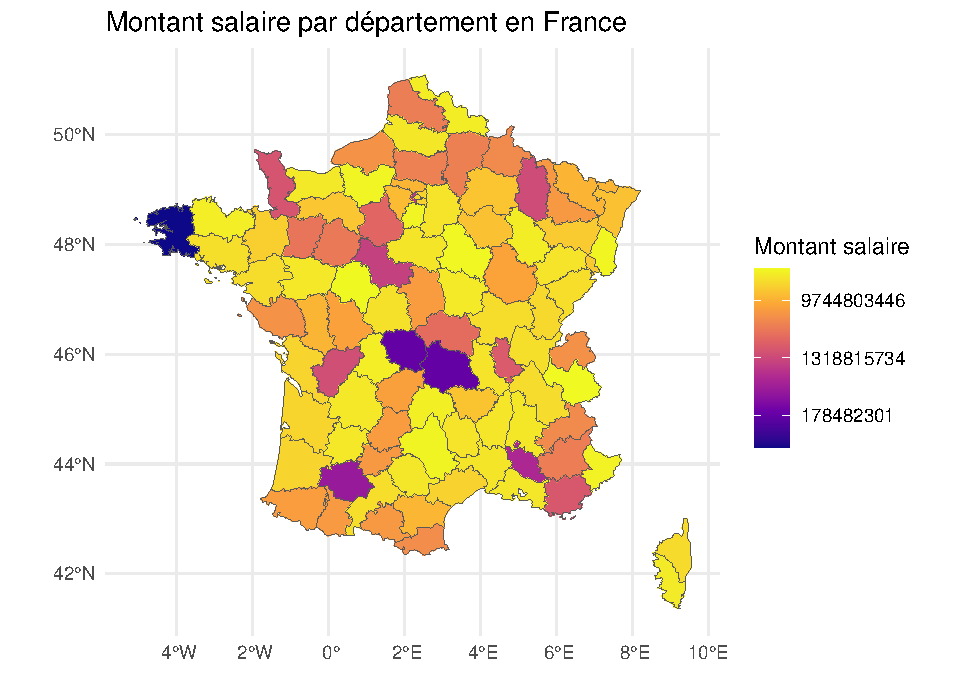
\includegraphics[width=12cm]{GroupReportTemplate-2_files/figure-latex/unnamed-chunk-30-1} \end{center}

\section*{\texorpdfstring{\textbf{Codes}}{Codes}}\label{codes}
\addcontentsline{toc}{section}{\textbf{Codes}}

\begin{figure}
\centering
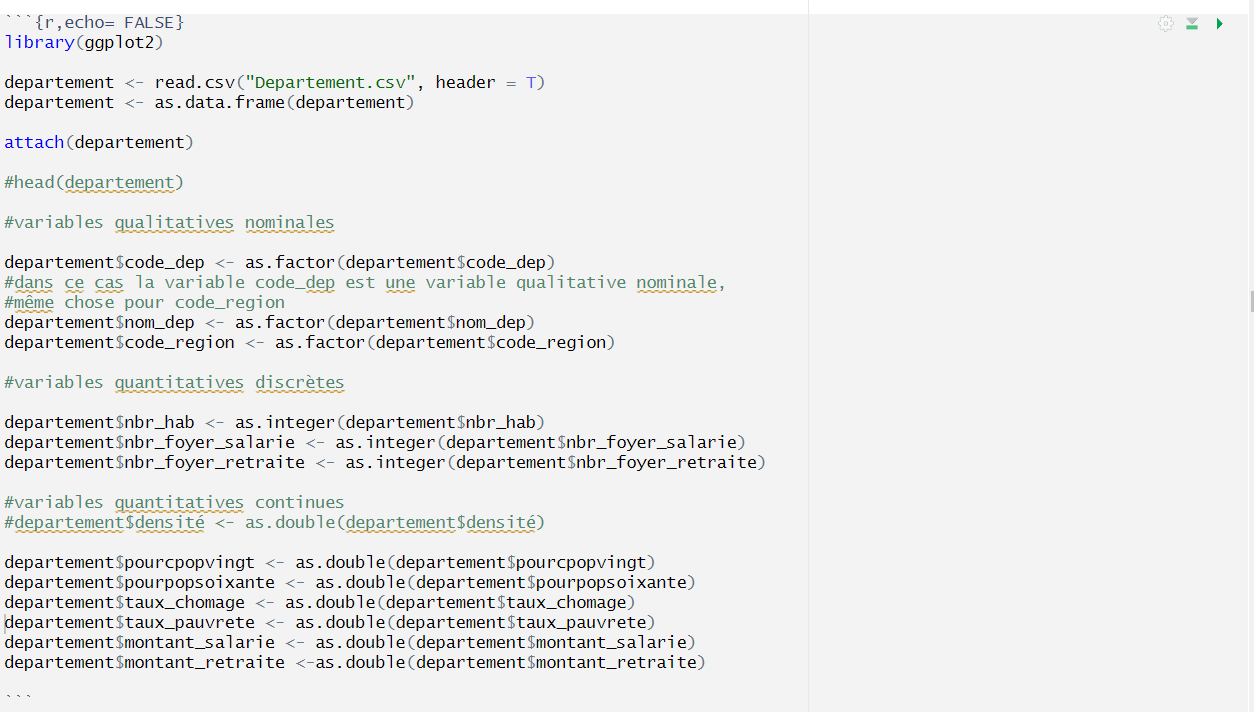
\includegraphics[width=15cm,height=10cm]{Images/Nature_var_dep.png}
\caption{Code de la nature des variables dans la table
Departement.}\label{Nature}
\end{figure}

\medskip 

\begin{figure}
\centering
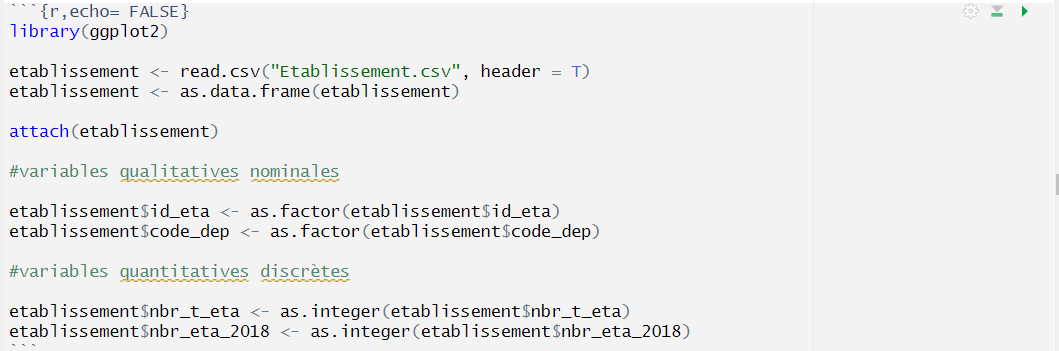
\includegraphics[width=15cm,height=9cm]{Images/Nature_var_eta.png}
\caption{Code de la nature des variables dans la table
Etablissement.}\label{Nature}
\end{figure}

\medskip 

\begin{figure}
\centering
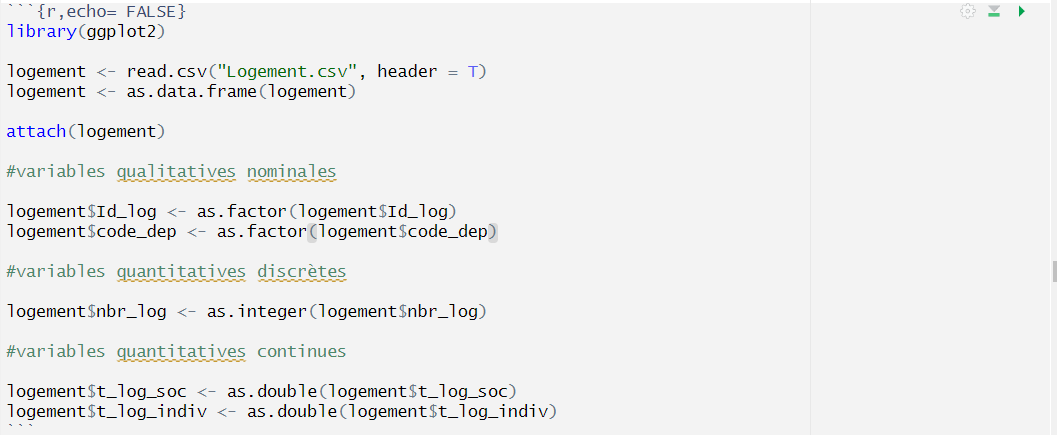
\includegraphics[width=15cm,height=9cm]{Images/Nature_var_log.png}
\caption{Code de la nature des variables dans la table
Logement.}\label{Nature}
\end{figure}

\medskip 

\begin{figure}
\centering
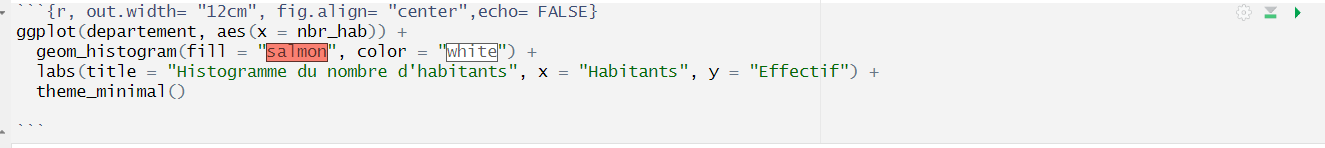
\includegraphics[width=15cm,height=2cm]{Images/hist_nbr_hab.png}
\caption{Code de l'histogramme du nombre d'habitants par
département(nbr\_hab).}\label{Histogramme}
\end{figure}

\medskip

\begin{figure}
\centering
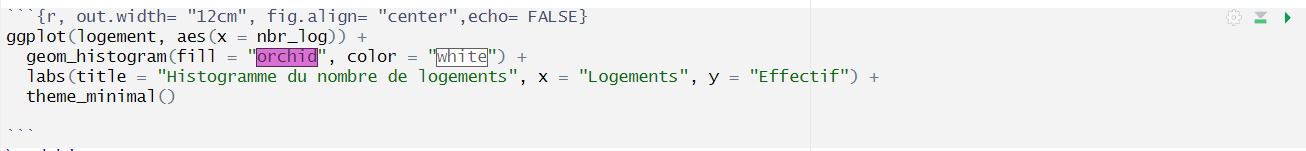
\includegraphics[width=15cm,height=2cm]{Images/hist_nbr_log.png}
\caption{Code de l'histogramme du nombre de logements par
département(nbr\_log).}\label{Histogramme2}
\end{figure}

\medskip

\begin{figure}
\centering
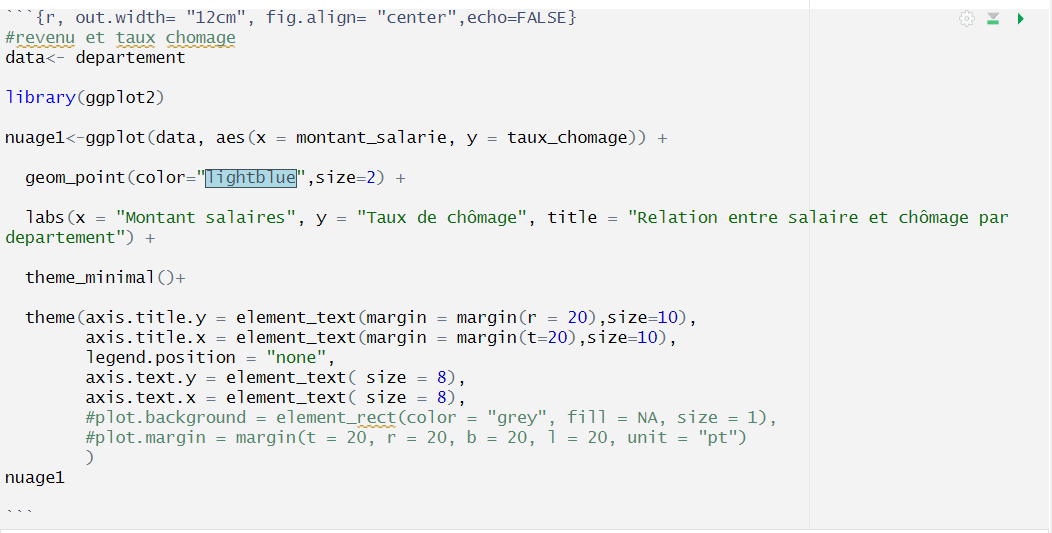
\includegraphics[width=15cm,height=9cm]{Images/Nuage_de_point_revenu_chomage.png}
\caption{Code du nuage de points entre les revenu des salaires et le
taux de chômage .}\label{Nuage}
\end{figure}

\medskip

\begin{figure}
\centering
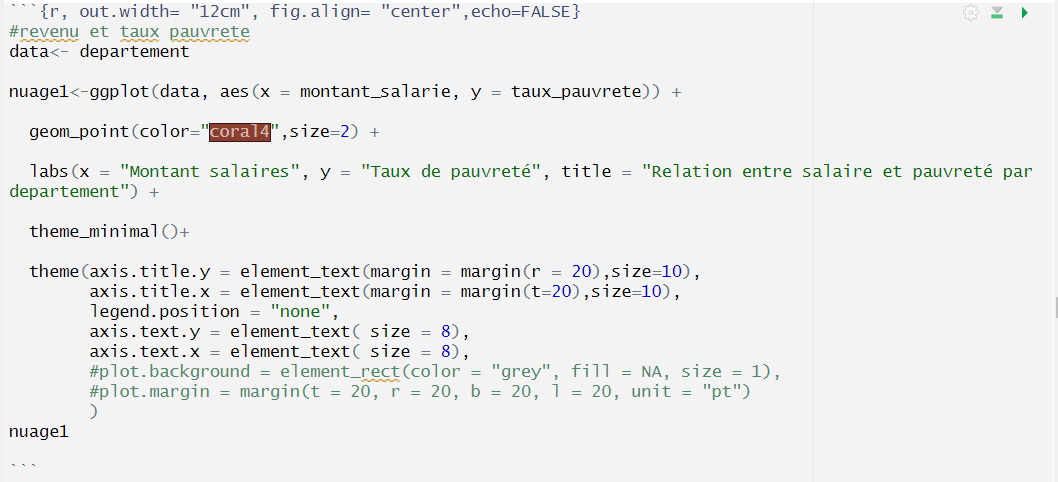
\includegraphics[width=15cm,height=9cm]{Images/Nuage_de_point_revenu_pauvrete.png}
\caption{Code du nuage de points entre les revenu des salaires et le
taux de pauvreté .}\label{Nuage}
\end{figure}

\medskip

\begin{figure}
\centering
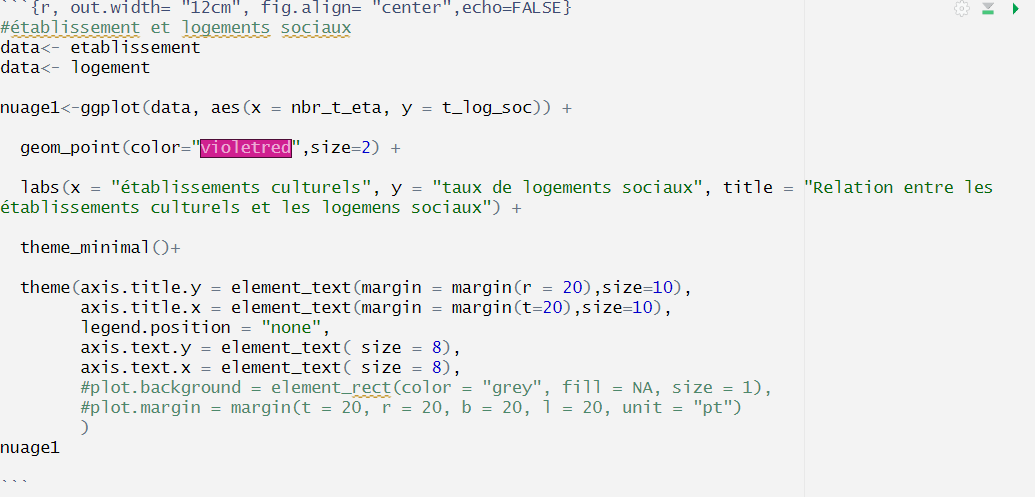
\includegraphics[width=15cm,height=9cm]{Images/Nuage_de_point_tauxlog_t_eta.png}
\caption{Code du nuage de points entre le taux de logements sociaux et
le nombre total d'établissement .}\label{Nuage}
\end{figure}

\medskip

\begin{figure}
\centering
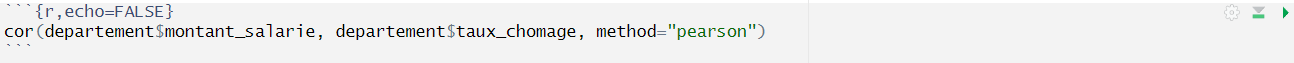
\includegraphics[width=15cm,height=1cm]{Images/coeff_cor.png}
\caption{Code d'un exemple de coefficient de corrélation
.}\label{Correlation}
\end{figure}

\medskip

\begin{figure}
\centering
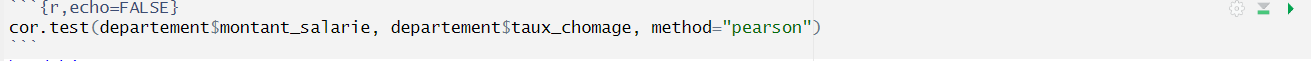
\includegraphics[width=15cm,height=1cm]{Images/test_cor.png}
\caption{Code d'un exemple de test de corrélation .}\label{Test_corr}
\end{figure}

\medskip

\begin{figure}
\centering
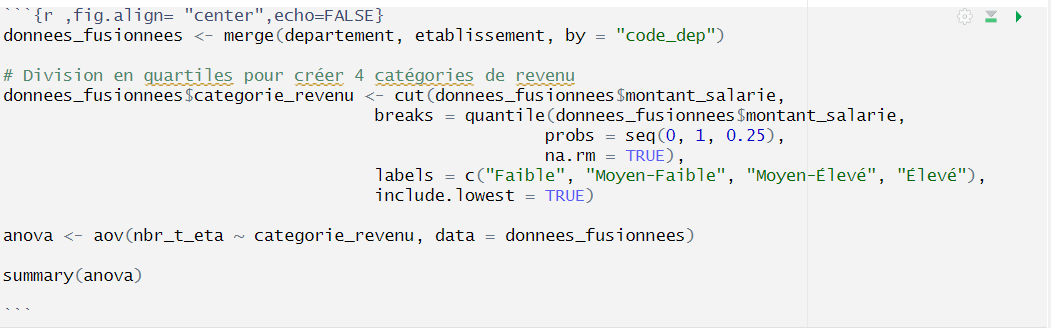
\includegraphics[width=15cm,height=5cm]{Images/test_anova.png}
\caption{Code du test d'ANOVA .}\label{ANOVA}
\end{figure}

\medskip

\begin{figure}
\centering
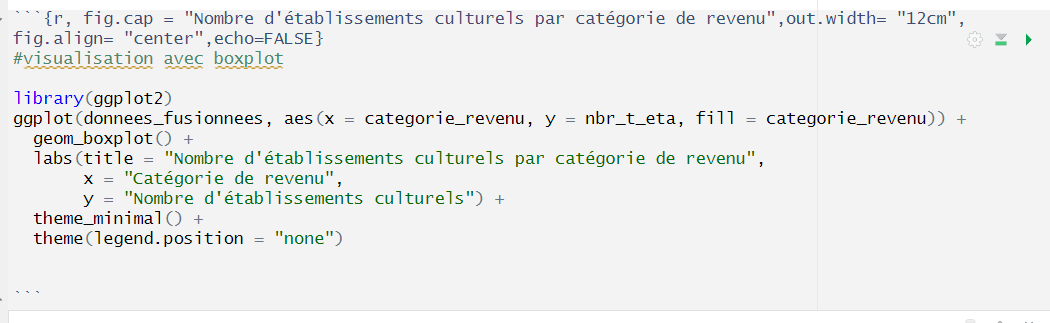
\includegraphics[width=15cm,height=5cm]{Images/box_plot.png}
\caption{Code du box-plot.}\label{Box_plot}
\end{figure}







\end{document}

